\documentclass[12pt,letterpaper]{article}
\usepackage[utf8]{inputenc}
\usepackage[spanish]{babel}
\usepackage{graphicx}
\usepackage[left=2cm,right=2cm,top=2cm,bottom=2cm]{geometry}
\usepackage{graphicx} % figuras
% \usepackage{subfigure} % subfiguras
\usepackage{float} % para usar [H]
\usepackage{amsmath}
%\usepackage{txfonts}
\usepackage{stackrel} 
\usepackage{multirow}
\usepackage{enumerate} % enumerados
\renewcommand{\labelitemi}{$-$}
\renewcommand{\labelitemii}{$\cdot$}
% \author{}
% \title{Caratula}
\begin{document}

% Fancy Header and Footer
% \usepackage{fancyhdr}
% \pagestyle{fancy}
% \cfoot{}
% \rfoot{\thepage}
%

% \usepackage[hidelinks]{hyperref} % CREA HYPERVINCULOS EN INDICE

% \author{}
\title{Caratula}

\begin{titlepage}
\begin{center}
\large{UNIVERSIDAD PRIVADA-DE-TACNA}\\
\vspace*{-0.025in}
\begin{figure}[htb]
\begin{center}

\includegraphics[width=8cm]{./Imagenes/logo}
\end{center}
\end{figure}
\vspace*{0.15in}
INGENIERIA DE SISTEMAS  \\

\vspace*{0.5in}
\begin{large}
TITULO:\\
\end{large}

\vspace*{0.1in}
\begin{Large}
\textbf{TRABAJO ENCARGADO No 02} \\
\end{Large}

\vspace*{0.3in}
\begin{Large}
\textbf{CURSO:} \\
\end{Large}

\vspace*{0.1in}
\begin{large}
BASE DE DATOS II\\
\end{large}

\vspace*{0.3in}
\begin{Large}
\textbf{DOCENTE(ING):} \\
\end{Large}

\vspace*{0.1in}
\begin{large}
 Patrick Cuadros Quiroga\\
\end{large}

\vspace*{0.2in}
\vspace*{0.1in}
\begin{large}
Integrantes: \\
\begin{flushleft}
J		\hfill	(201) \\
Samuel Ray Núñez Mamani 		\hfill	(2016054462) \\
Andre Sebastian Reinoso Aranda          	\hfill	(2016055275) \\
M      	\hfill	(201) \\

\end{flushleft}
\end{large}
\end{center}

\end{titlepage}





\documentclass[twoside,twocolumn]{article}

\usepackage{blindtext} % Package to generate dummy text throughout this template 
\usepackage{graphicx}
\usepackage[sc]{mathpazo} % Use the Palatino font
\usepackage[T1]{fontenc} % Use 8-bit encoding that has 256 glyphs
\linespread{1.05} % Line spacing - Palatino needs more space between lines
\usepackage{microtype} % Slightly tweak font spacing for aesthetics

\usepackage[english]{babel} % Language hyphenation and typographical rules

\usepackage[hmarginratio=1:1,top=32mm,columnsep=20pt]{geometry} % Document margins
\usepackage[hang, small,labelfont=bf,up,textfont=it,up]{caption} % Custom captions under/above floats in tables or figures
\usepackage{booktabs} % Horizontal rules in tables

\usepackage{lettrine} % The lettrine is the first enlarged letter at the beginning of the text

\usepackage{enumitem} % Customized lists
\setlist[itemize]{noitemsep} % Make itemize lists more compact

\usepackage{abstract} % Allows abstract customization
\renewcommand{\abstractnamefont}{\normalfont\bfseries} % Set the "Abstract" text to bold
\renewcommand{\abstracttextfont}{\normalfont\small\itshape} % Set the abstract itself to small italic text

\usepackage{titlesec} % Allows customization of titles
\renewcommand\thesection{\Roman{section}} % Roman numerals for the sections
\renewcommand\thesubsection{\roman{subsection}} % roman numerals for subsections
\titleformat{\section}[block]{\large\scshape\centering}{\thesection.}{1em}{} % Change the look of the section titles
\titleformat{\subsection}[block]{\large}{\thesubsection.}{1em}{} % Change the look of the section titles

\usepackage{fancyhdr} % Headers and footers
\pagestyle{fancy} % All pages have headers and footers
\fancyhead{} % Blank out the default header
\fancyfoot{} % Blank out the default footer
\fancyhead[C]{Titulo $\bullet$ Junio 2019 $\bullet$ } % Custom header text
\fancyfoot[RO,LE]{\thepage} % Custom footer text

\usepackage{titling} % Customizing the title section

\usepackage{hyperref} % For hyperlinks in the PDF

%----------------------------------------------------------------------------------------
%	TITLE SECTION
%----------------------------------------------------------------------------------------

\setlength{\droptitle}{-4\baselineskip} % Move the title up

\pretitle{\begin{center}\Huge\bfseries} % Article title formatting
\posttitle{\end{center}} % Article title closing formatting
\title{Virtualizacion y Contenedores} % Article title
\author{Andre Reinoso, Samuel Nuñez, Andres De la Barra ,David Damian y Richard Cruz}
\date{\today} % Leave empty to omit a date
\renewcommand{\maketitlehookd}{%
\begin{abstract}
\noindent Ingles
\end{abstract}
\begin{abstract}
\noindent Español.
\end{abstract}
}

%----------------------------------------------------------------------------------------

\begin{document}

% Print the title
\maketitle

%----------------------------------------------------------------------------------------
%	ARTICLE CONTENTS
%----------------------------------------------------------------------------------------

\section{Introduccion}

\lettrine[nindent=0em,lines=3]{L}a virtualiza



%------------------------------------------------

\section{Objetivos}

\begin{itemize}
\item Entender qué es una máquina virtual.
\item Entender qué es un contenedor.
\item Comparar ambos conceptos.
\item Establecer un juicio acerca de las ofertas y el potencial de ambas.

\end{itemize}




%------------------------------------------------

\section{Desarrollo}

\subsection{¿Que es una maquina virtual?}

Una máquina virtual 

\begin{center}
	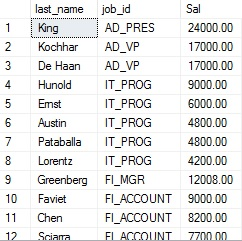
\includegraphics[width=5cm]{./Imagenes/virtualizacion} 
	\end{center}




\subsection{¿Que es un contenedor?}

Los cont

\begin{itemize}
\item Docker
\\ Éste con




\begin{center}
	
\includegraphics[width=5cm]{./Imagenes/docker} 
	\end{center}

Ventajas
\\ \textbf{- Las instancias se inician en pocos segundos.}


Desventajas
\\ \textbf{- Sólo puede usarse de forma nativa en entornos Unix con Kernel igual o superior a 3.8.}
\end{itemize} 

\subsection{¿Diferencia entre maquinas virtuales y contenedores?}
El objetivo pri

\begin{itemize}
	\item Jerarquia maquina virtual
	\\La primer gran diferencia es la jerarquia, forma de como estan constituidas. En el primero de los casos las maquinas virtuales estan constituidas por:

	\begin{center}
	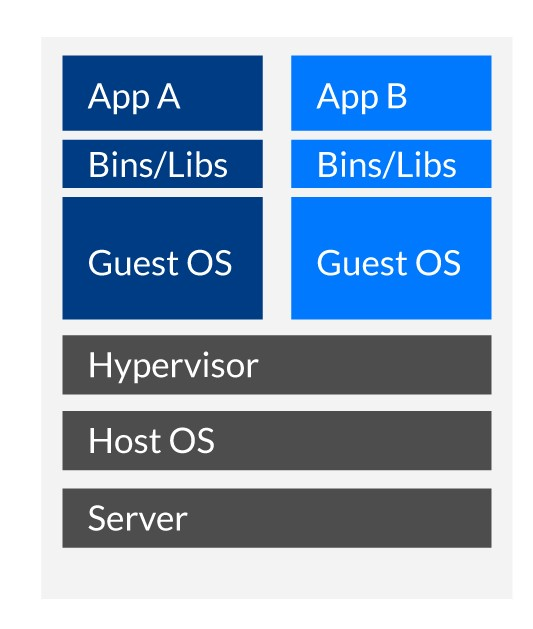
\includegraphics[width=5cm]{./Imagenes/jerarquia1} 
	\end{center}
\end{itemize} 

\begin{itemize}
	\item Jerarquia contenedor
	\\ \textbf{-El servidor o una computador}.

	\begin{center}
	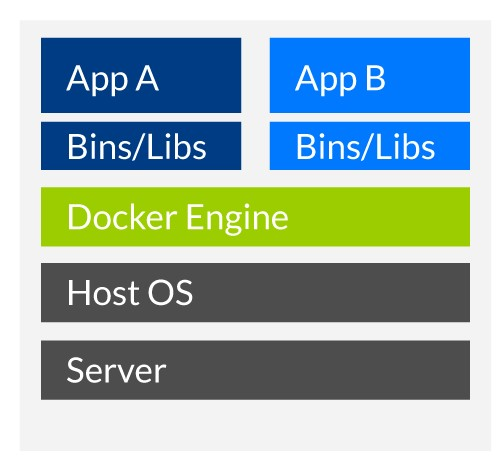
\includegraphics[width=5cm]{./Imagenes/jerarquia2} 
	\end{center}
\end{itemize} 

\begin{itemize}
	\item Los contenedores permiten desplegar aplicaciones más rápido, arrancarlas y pararlas más rápido y aprovechar mejor los recursos de hardware.




\end{itemize} 

\section{Conclusiones}

Para hablar de contenedores y
%	REFERENCE LIST
%----------------------------------------------------------------------------------------

\begin{thebibliography}{99} % Bibliography - this is intentionally simple in this template

\bibitem[Martin, 2011]{Diego Martin:2011dg}
Martin, M.M,  y J.U (2011).
\newblock Virtualización, una solución para la eficiencia,
seguridad y administración de intranets
\newblock {\em El profesional de la informacion}, 350.
\newblock Contenedor de aplicaciones: Docker (2015)
 
 
\end{thebibliography}

%----------------------------------------------------------------------------------------

\end{document}




\end{document}
